\scanpage{40}\mspage{39}
% @axiom
\uline{Cont} 5 Let $X.Y\in M$, $X$ and $Y$ \uline{disjoint}. Then for $X'\ll X$ and $Y'\ll Y$, $X'$ and $Y'$ are \deleted{disjoint} \deleted{compatible} disjoint
\margin{
\begin{tikzpicture}[x=1cm,y=1cm]\draw (0,0)--(-.03,1.7) (.08,.05)--(.05,1.8) (.16,.08)--(.13,1.8);\draw (-.25,1.95)--(.1,2.2)--(.05,2.4)--(.18,2.24)--(.35,2.32);\end{tikzpicture}}
% @sim
% slanted
\margin{Is akin to \uline{Cont} 2 (page 33)}
% @cancelone

\figure{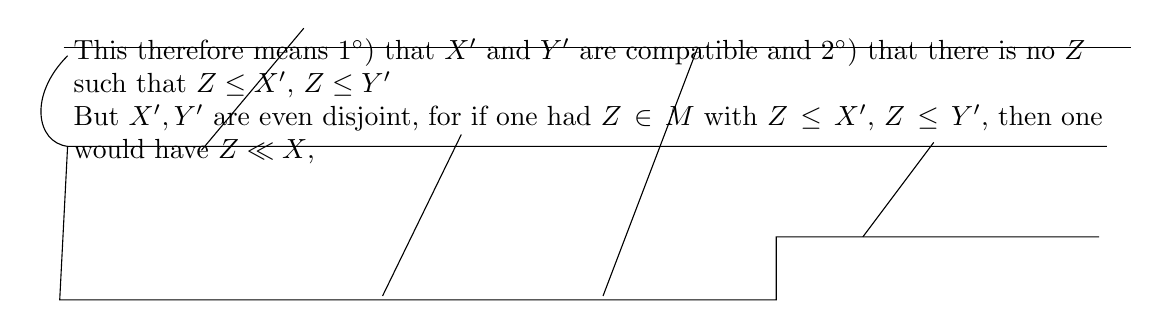
\begin{tikzpicture}[x=1cm,y=1cm]
\node[anchor=north west,inner sep=2pt,text width=13.5cm] (cancelled) at (0,0) {\deleted{This therefore means $1^\circ$) that $X'$ and $Y'$ are compatible and $2^\circ$) that there is no $Z$ such that $Z\leq X'$, $Z\leq Y'$}
% @canceltwo

\deleted{But $X',Y'$ are even disjoint, for if one had \inserted{$Z\in M$ with} $Z\leq X'$, $Z\leq Y'$, then one would have $Z\ll X$,}};
\draw (-.05,-.2)--(13.5,-.2);
\draw (0,-.3) .. controls (-.5,-.8) and (-.4,-1.4) .. (0,-1.45)--(13.2,-1.45);
\draw (0,-1.45)--(-.1,-3.4)--(9,-3.4)--(9,-2.6)--(13.1,-2.6);
\draw (3,.05)--(1.7,-1.5) (5,-1.3)--(4,-3.35) (8,-.2)--(6.8,-3.35) (11,-1.4)--(10.1,-2.6);
\end{tikzpicture}}
% @split

Decomposes into two

% @splita
\textcircled{\scriptsize a} Under the condition of Cont 5, $X'$ and $Y'$ are \uline{compatible}
% @noz

\textcircled{\scriptsize b} \deleted{If $Z$} $\nexists\ Z\in M$ with $Z\ll X$, $Z\ll\deleted{X}Y$.
% @ip

(i.e if $X,Y$ compatible, then $M_{\leq\unsure{x|X}}\cap M_{\leq Y}=\varnothing$ even implies $M_{\ll X}\cap M_{\ll Y}=\varnothing$)
% @cor

\uline{Corollary} If $\unsure{F|\mathcal F}$ and $\unsure{G|\mathcal G|\mathbb G}$ are disjoint figures, then for every refinement $F'$ of $F$ and every refinement $G'$ of $G$, $F'$ and $G'$ are disjoint.
% @addcor
% slanted
\margin{\uline{Corollary} For two figures \deleted{\unsure{$F,G$}} $F,G$ to be disjoint, it is necessary and sufficient that for all $x\in\widetilde F,y\in\widetilde G$, that $x$ and $y$ disjoint}
% @remark

\uline{Remark} Let $M'$ be a subcountry. For two figures $F,G$ of $M'$, \deleted{their} \inserted{or two \unsure{multi-forms|multistrata} $X.Y$} to say that they are disjoint in the sense of $M'$ or of $M$ is the same, and likewise for the notion that $F$ refines $G$ If $M$ satisfies \uline{Cont} 5, $M'$ too. \inserted{it\deleted{\unsure{ou|em}} for \uline{Cont} 6 which follows}
\margin{\begin{tikzpicture}[x=1cm,y=1cm]\draw (0,.6) .. controls (-.2,.2) and (.2,.1) .. (1.1,.1) .. controls (1.6,.1) and (1.5,-.2) .. (1.65,-.5)--(1.9,-.2);\end{tikzpicture}}
% @six

\uline{Cont 6} (Optional ?) If $X$ and, $Y\in M$ are such that \deleted{$\forall$} $\widetilde X\cap\widetilde Y=\varnothing$ \uuline{and} every $a\in\widetilde X$ is compatible with \deleted{\unsure{every|all}} $y\in\widetilde Y$, then $X$ and $Y$ are disjoint
% @foot
\margin{\tikz[baseline]{\draw[<->] (0,.68)--(.52,.20); \draw (.58,-.13)--(.58,.30) (.63,-.13)--(.63,.30) (.68,-.13)--(.68,.30); \draw (-.08,-.05) ellipse (.035 and .06); \draw (-.08,-.05)--(-.05,.26);}\,\unsure{with|therefore} every element $\unsure{\bar X|\widetilde X|x}$ disjoint from every $y\in\widetilde Y$}
